\section{Analyse von Regelsystemen}
    \subsection{Signale im Regelkreis}
    \begin{tabular}{l|l}
    $\mathbf{r(t)}$& Referenz (Sollzustand des Systems)\\
    $\mathbf{w(t)}$& Störung der Eingangsgrösse $u$\\
    $\mathbf{d(t)}$& Störung der Ausgangsgrösse $y$\\
    $\mathbf{n(t)}$& Sensorrauschen\\
    $\mathbf{e(t)}$& Regelfehler\\
    $\mathbf{y(t)}$& Ist-Wert/Ausgangsgrösse\\
    $\mathbf{u(t)}$& Stellgrösse\\
    \end{tabular}
    
    \begin{center}
        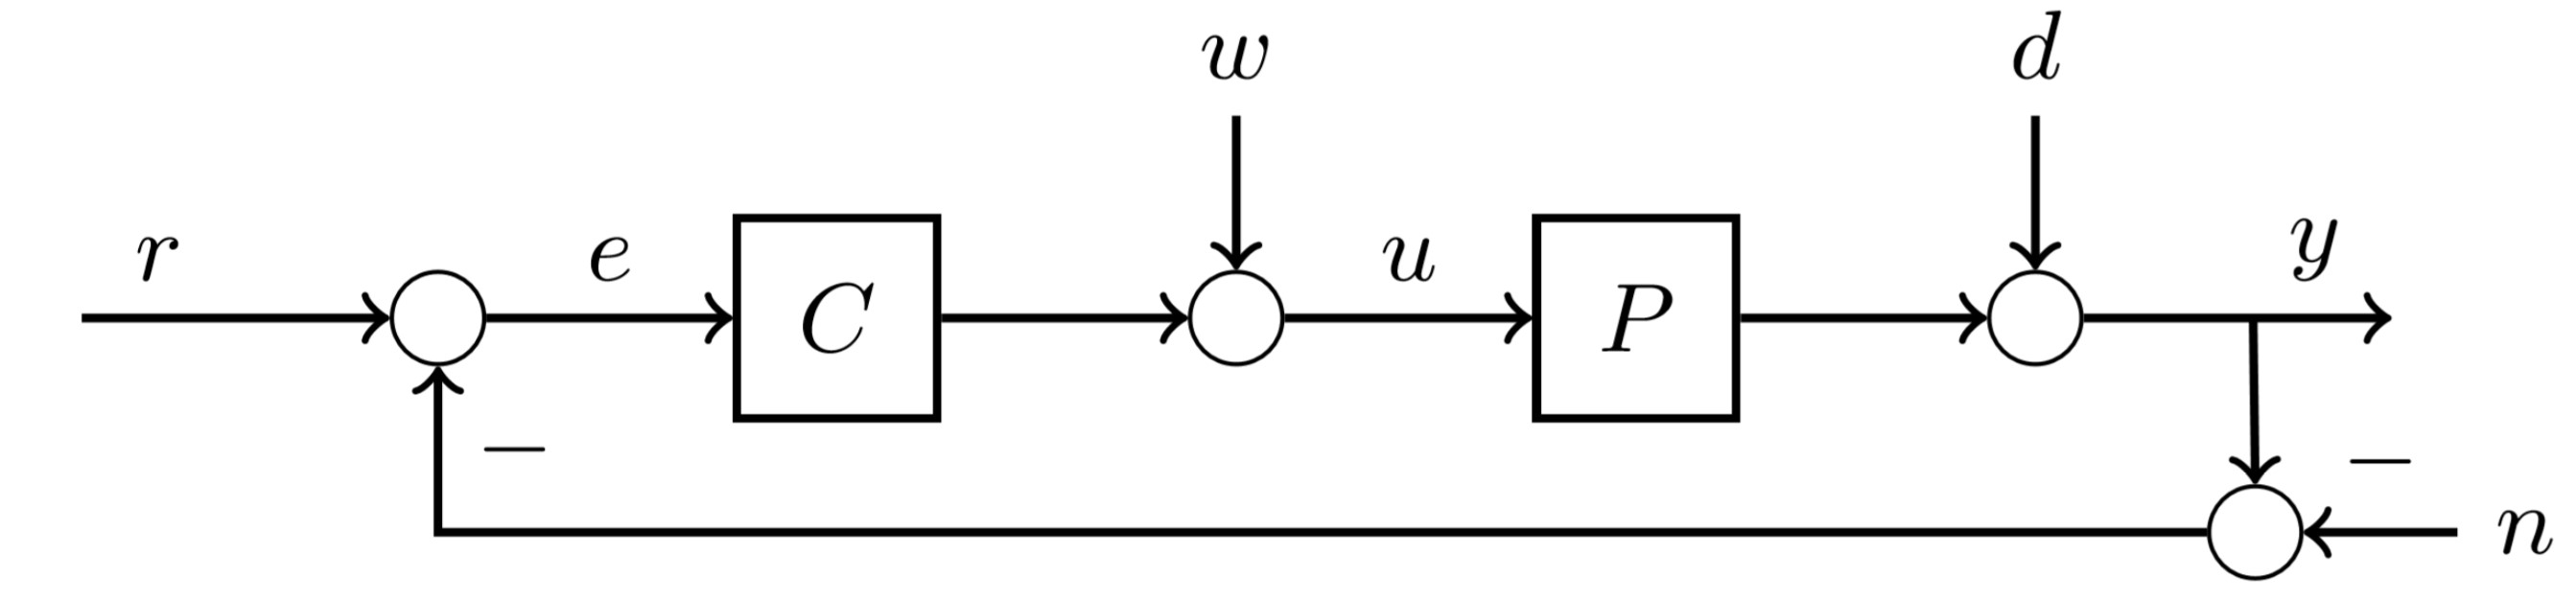
\includegraphics[width = 0.8\linewidth]{07/Standart_Regelkreis.jpg}
    \end{center}
    
    Um die Beziehung zwischen zwei beliebigen Signalen zu beschreiben. wird der Regelkreis zuerst in den Frequenzbereich transformiert:

    \begin{center}
        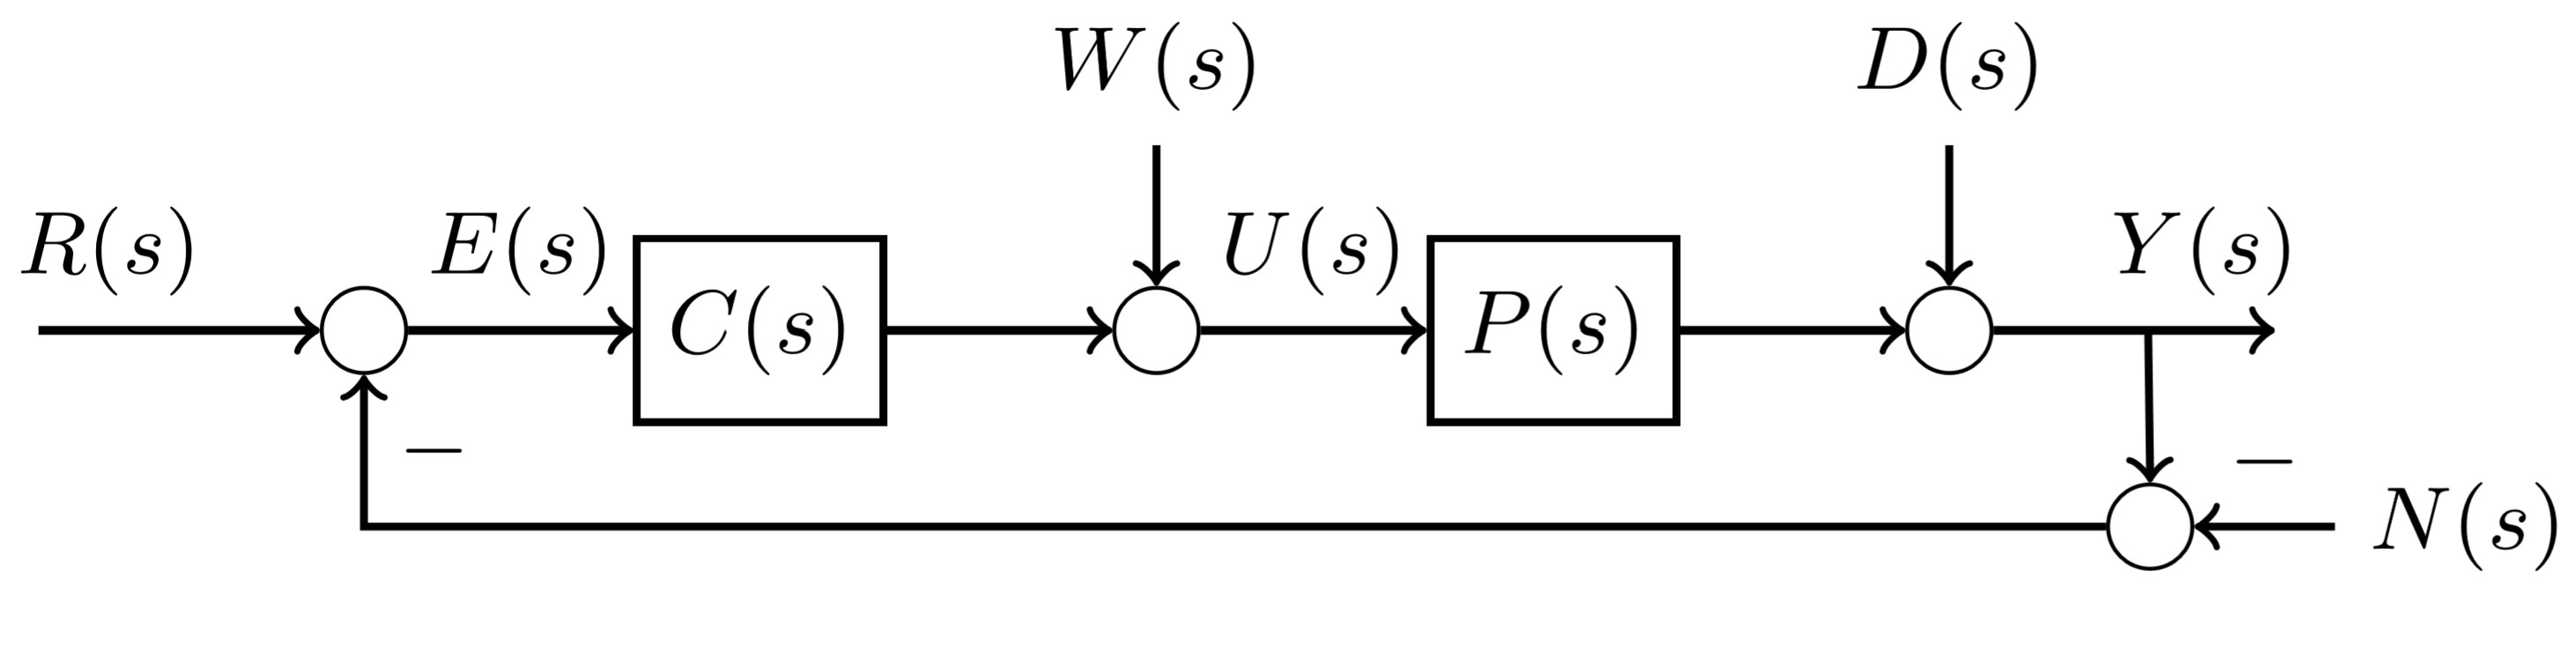
\includegraphics[width = 0.8\linewidth]{images/07/Standart_Regelkreis_FB.jpg}
    \end{center}
    
    Dabei soll die \textbf{Ausgangsgrösse} $Y(s)$ als Funktion des \textbf{Reglers} $C(s)$, der \textbf{Regelstrecke} $P(s)$ und der \textbf{Eingänge} $R(s)$, $N(s)$, $D(s)$, und $W(s)$ geschrieben werden.
    Durch die Linearität der Regelstruktur und Annahme von unkorrelierten Eingängen können die Eingangsbeiträge einzeln betrachtet werden.
    
    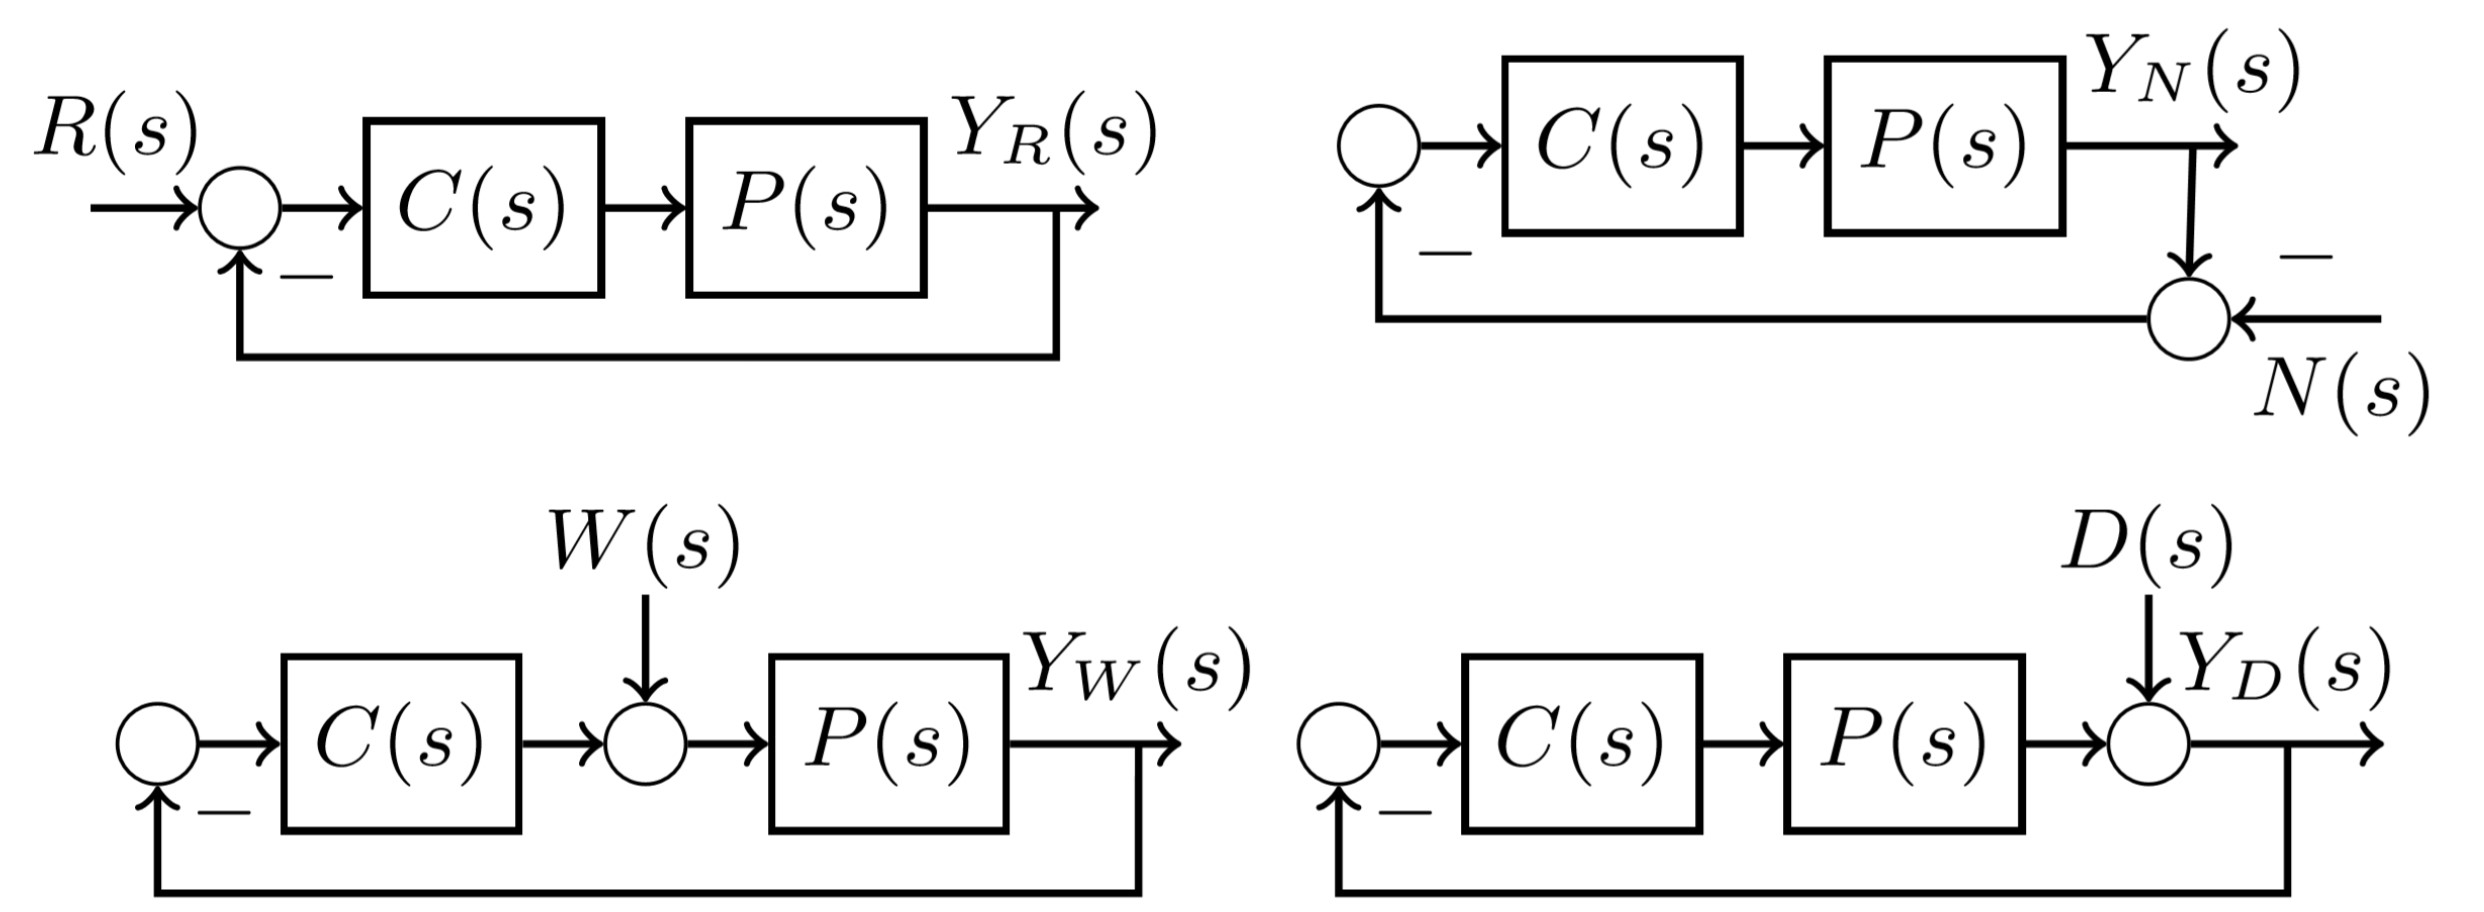
\includegraphics[width = \linewidth]{images/07/Eingangsbeitraege.jpg}
    
    Daraus folgt: 
    \[\begin{matrix}
    Y_R(s) = \frac{P(s)C(s)}{1+P(s)C(s)}\cdot R(s), & Y_N(s) = \frac{P(s)C(s)}{1+P(s)C(s)}\cdot N(s) \\
    &\\
    Y_W(s) = \frac{P(s)}{1+P(s)C(s)}\cdot W(s), &
    Y_D(s) =  \frac{1}{1+P(s)C(S)}\cdot D(s)  

    \end{matrix}\]
    
    Die gesamte Ausgangsgrösse $Y(s)$ lautet somit:
    \[
    Y(s) = Y_R(s) + Y_N(s)+Y_W(s)+ Y_D(s)
    \]
    
    Es Werde folgende Komponenten definiert:
    
    {\renewcommand{\arraystretch}{1.5}
    \begin{tabular}{l|c|c}
    
    \textbf{Kreisverstärkung}    &$L(s)=P(s) C(s)$   & $(e\rightarrow y)$ \\
     \textbf{Sensititvität}  & $S(s) = \frac{1}{1+L(s)}$  & ($d\rightarrow y$, $r\rightarrow e$)   \\ 
     \multirow{2}{10em}{
      \textbf{Komplementäre} \textbf{Sensitivität}} & &\\& $T(s) = \frac{L(s)}{1+L(s)}$ &($r\rightarrow y$, $n\rightarrow y$)
      
        
    \end{tabular}
    }
    Grundsätzlich gilt: \[\textrm{übertragungsfunktion}=\frac{\textrm{Vorwärtspfad}}{1+\textrm{Kreisverstärkung}}\]
    
    \subsection{Stabilität des geschlossenen Regelkreises}
        Für geschlossene Regelkreise muss das Konzept der Stabilität erweitert werden. Ein System ist \textbf{intern stabil}, wenn \textit{alle} Übertragungsfunktionen, welche die Eingänge \textit{w, d, r} im Regelkreis auf die Ausgänge \textit{u, y, e} abbilden, asymptotisch stabil sind ($\textrm{Re}(\lambda_i)<0,\forall i=1,\dots n)$. Die Beziehungen sind durch diese Matrix gegeben:
        \[\begin{bmatrix}
        U(s)\\Y(s)\\E(s)
        \end{bmatrix}
        =
        \begin{bmatrix}
        S(s)    &   -S(s)\cdot C(s) &   S(s)\cdot C(s)\\
        S(s)\cdot P(s)  &   S(s)    &   T(s)\\
        -S(s)\cdot P(s) &   -S(s)   &   S(s)
        \end{bmatrix}
        \cdot
        \begin{bmatrix}
        W(s)\\D(s)\\R(s)
        \end{bmatrix}
        \]
        $\Rightarrow S(s),T(s),S(s)\cdot C(s), S(s)\cdot P(s)$ dürfen nur asymptotisch stabile Pole haben.
        
        Falls $P(s)$ und $C(s)$ nur asymptotisch stabile Pole haben, genügt es also, die asymptotische Stabilität von $S(s)$ oder $T(s)$ zu überprüfen um interne Stabilität zu garantieren.
        
        Wenn wir nur an $r\rightarrow y$ interessiert sind darf das \textbf{charakteristische Polynom} $1+L(s)=0$ nur NST mit $Re(\zeta)<0$ haben. (Falls $C(s)$ oder $P(s)$ instabile Pole haben muss interne Stabilität separat noch überprüft werden.)
        %\TODO{Interne Stabilität muss nur geprüft werden, wenn P oder C instabile Pole hat, sonst genügt es, die Nullstellen von 1+L(s) zu überprüfen. von RT.. stimmt das? chonnt mer vonere üebigsstond bekannt vor.. mösst aber nomol nacheluege}


    \subsection{Nyquist Theorem}
            Durch das Nyquist Theorem kann die asymptotische Stabilität eines geschlossenen Regelkreissystems $T(s)=\frac{L(s)}{1+L(s)}$ durch Analyse seiner Kreisverstärkung $L(s)$ (offener Regelkreis) bestimmt werden. Dabei wird angenommen, dass keine Modellunsicherheit $W_2(s)$ vorhanden ist.
% \vfill\null\columnbreak            
        \subsubsection{Nominelles Stabilitätskriterium von Nyquist}
            Der geschlossene Regelkreis mit Übertragungsfunktion $T(s)$ ist asymptotisch stabil, falls für $L(s)$ gilt:
            \[n_c\overset{!}{=}\frac{n_0}{2}+n_+\]
            \begin{tabular}{l l}
                $n_c$:  & Anzahl Umrundungen um den kritischen Punkt (-1,0)  \\
                        & Positiv falls Umrundung gegen Uhrzeigersinn.\\
                $n_0$:  & Anzahl Pole von $L(s)$ mit Realteil = 0\\
                $n_+$:  & Anzahl Pole von $L(s)$ mit Realteil $>$ 0
            \end{tabular}
            \textbf{Wichtig:} Stabilität nach Nyquist gilt nur, falls \textbf{keine Kürzung von instabilen Polen mit nicht minimalphasigen NST auftreten} in $L(s)=C(s)\cdot P(s)$.
            Andernfalls kann nicht von $L(s)$ auf die interne Stabilität des geschlossenen Regelkreises geschlossen werden.
        \subsubsection{Vorgehen zu Auswertung des Stabilitätskriteriums}
            \begin{enumerate}
                \item Betrachte das Nyquist-Diagramm von $L(j\omega)$ in der komplexen Ebene mit $\omega\in 0,\infty)$.
                \item Spiegle das Diagramm um die reelle Achse. Die gespiegelte Kurve entspricht dem Bereich $\omega \ in (-\infty,0]$. die kombinierte Kurven entspricht also $L(j\omega)$, $\omega \in (-\infty,\infty)$
                \item Zähle $n_c$ die Anzahl Umrundungen von $L(j\omega)$ um den Punkt $(-1+j0)$ wenn $\omega$ von $-\infty$ bis $\infty$ variiert wird. Ein Umlauf in $\circlearrowleft$ wird positiv gezählt, und in $\circlearrowright$ negativ.
            \end{enumerate}
            
    \subsection{Verstärkung und Phasenreserve}
        \begin{wrapfigure}[10]{r}{0.4\linewidth}
        \vspace{-4mm}
            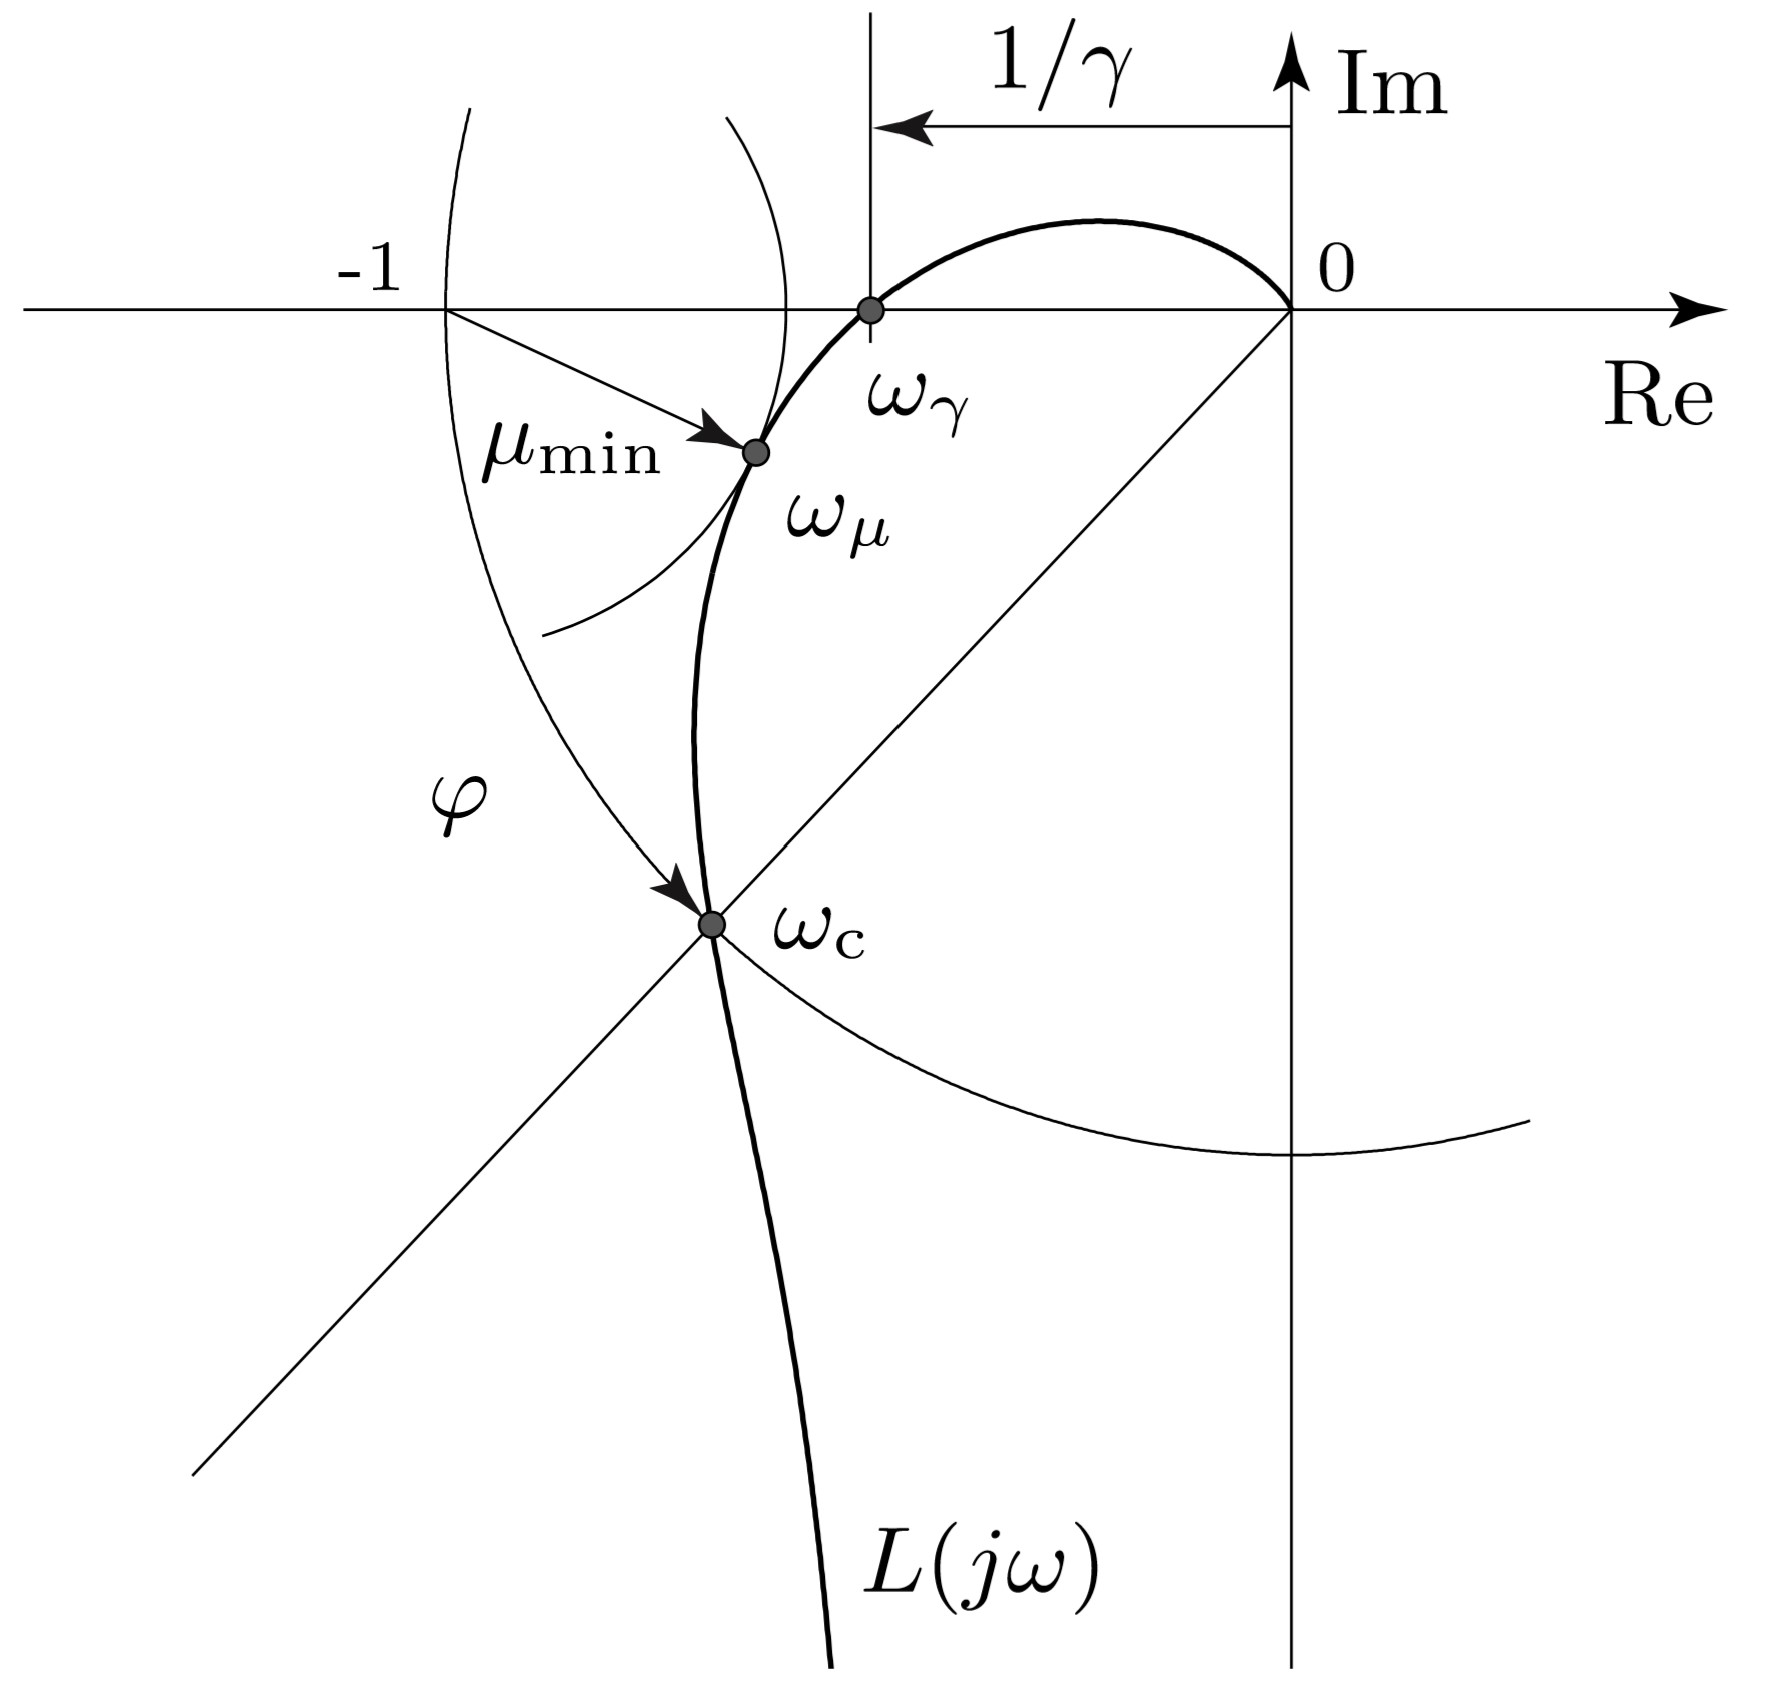
\includegraphics[width=\linewidth]{images/07/Robustheit.jpg}
        \end{wrapfigure}
        Falls $L(s)$ eines Systems das nominelle Stabilitätskriterium \textbf{nicht erfüllt}, hat das resultierende $T(s)=\frac{L(s)}{1+L(s)}$ instabile Pole. 
        
        Falls $L(s)$ eines Systems das nominale Stabilitätskriterium \textbf{erfüllt} kann mittels Verstärkungs- und Phasenreserve eine Aussage bezüglich der Stabilität (Robustheit) gemacht werden. 
\vfill\null\columnbreak
        Es werden drei Robustheitsmasse eingeführt:
        
        \begin{tabular}{|l|c|c|}
        \hline
        &&\\
        $\gamma$    & Verstärkungsreserve & \multirow{2}{14em}{Verstärkungsreserve zu $(-1+0j)$ bei $\angle L(j\omega) = -\pi$}\\
        &&\\
        \hline
        &&\\
        $\varphi$    & Phasenreserve& \multirow{2}{14em}{Phasenabstand zu $-\pi$ bei der Durchtrittsfrequenz $\omega_c$} \\
        &&\\
        \hline
        &&\\
        $\mu$ & kritische Abstand &\multirow{2}{14em}{Kleinste Distanz zwischen $(-1+0j)$ und $L(j\omega)$ } \\
        &&\\
        \hline
        \end{tabular}
        Phasenreserve bei instabilen Systemen nicht well defined
        \[\mu = min_{\mu} |1+L(j\omega)| = \frac{1}{max_\omega|S(j\omega)|}\]
        \subsubsection{Vorgehen um Phasenreserve herauszufinden}
        Um die Phasenreserve berechnen zu können, muss man die Phasen des offenen Regelkreises bei der Durchtrittsfrequenz berechnen.
        \begin{enumerate}
            \item Die Durchtrittsfrequenz durch Lösen der Gleichung $|C(j\omega_c)\cdot P(j\omega_c)| = 1$ 
            \item Nun wird die Phase bei der Durchtrittsfrequenz $\omega_c$ ausgerechnet. $\angle(L(j\omega_c)$
            \item Um die Phasenreserve auszurechnen wird $-\pi$ mit der soeben erhaltenen Phase bei der Durchtrittsfrequenz     subtrahiert
        \end{enumerate}
        
        \subsubsection{Bsp}
            Das nominelle System $L(s)$ hat Phasenfehler $\alpha$ oder Verstärkungsfehler $k$ gegenüber dem wahren System: 
            \[L_{t,\alpha}(s) = e^{-\alpha \cdot s / \omega_c}\cdot L(s), \hspace{4mm} L_{t,k}(s) = k\cdot L(s) \]
            $L_{t,\alpha}$ ist stabil für $\alpha <  \varphi$ und $L_{t,k}$ für $k<\gamma$. Falls beide Fehler gleichzeitig vorhanden sind, sind $\gamma$ und $\varphi$ keine guten Robustheitsmasse, Sie messen beide nur eindimensional.
                
        \subsection{Auslesen der Reserven bei Bode-Diagrammen}
            \begin{center}
                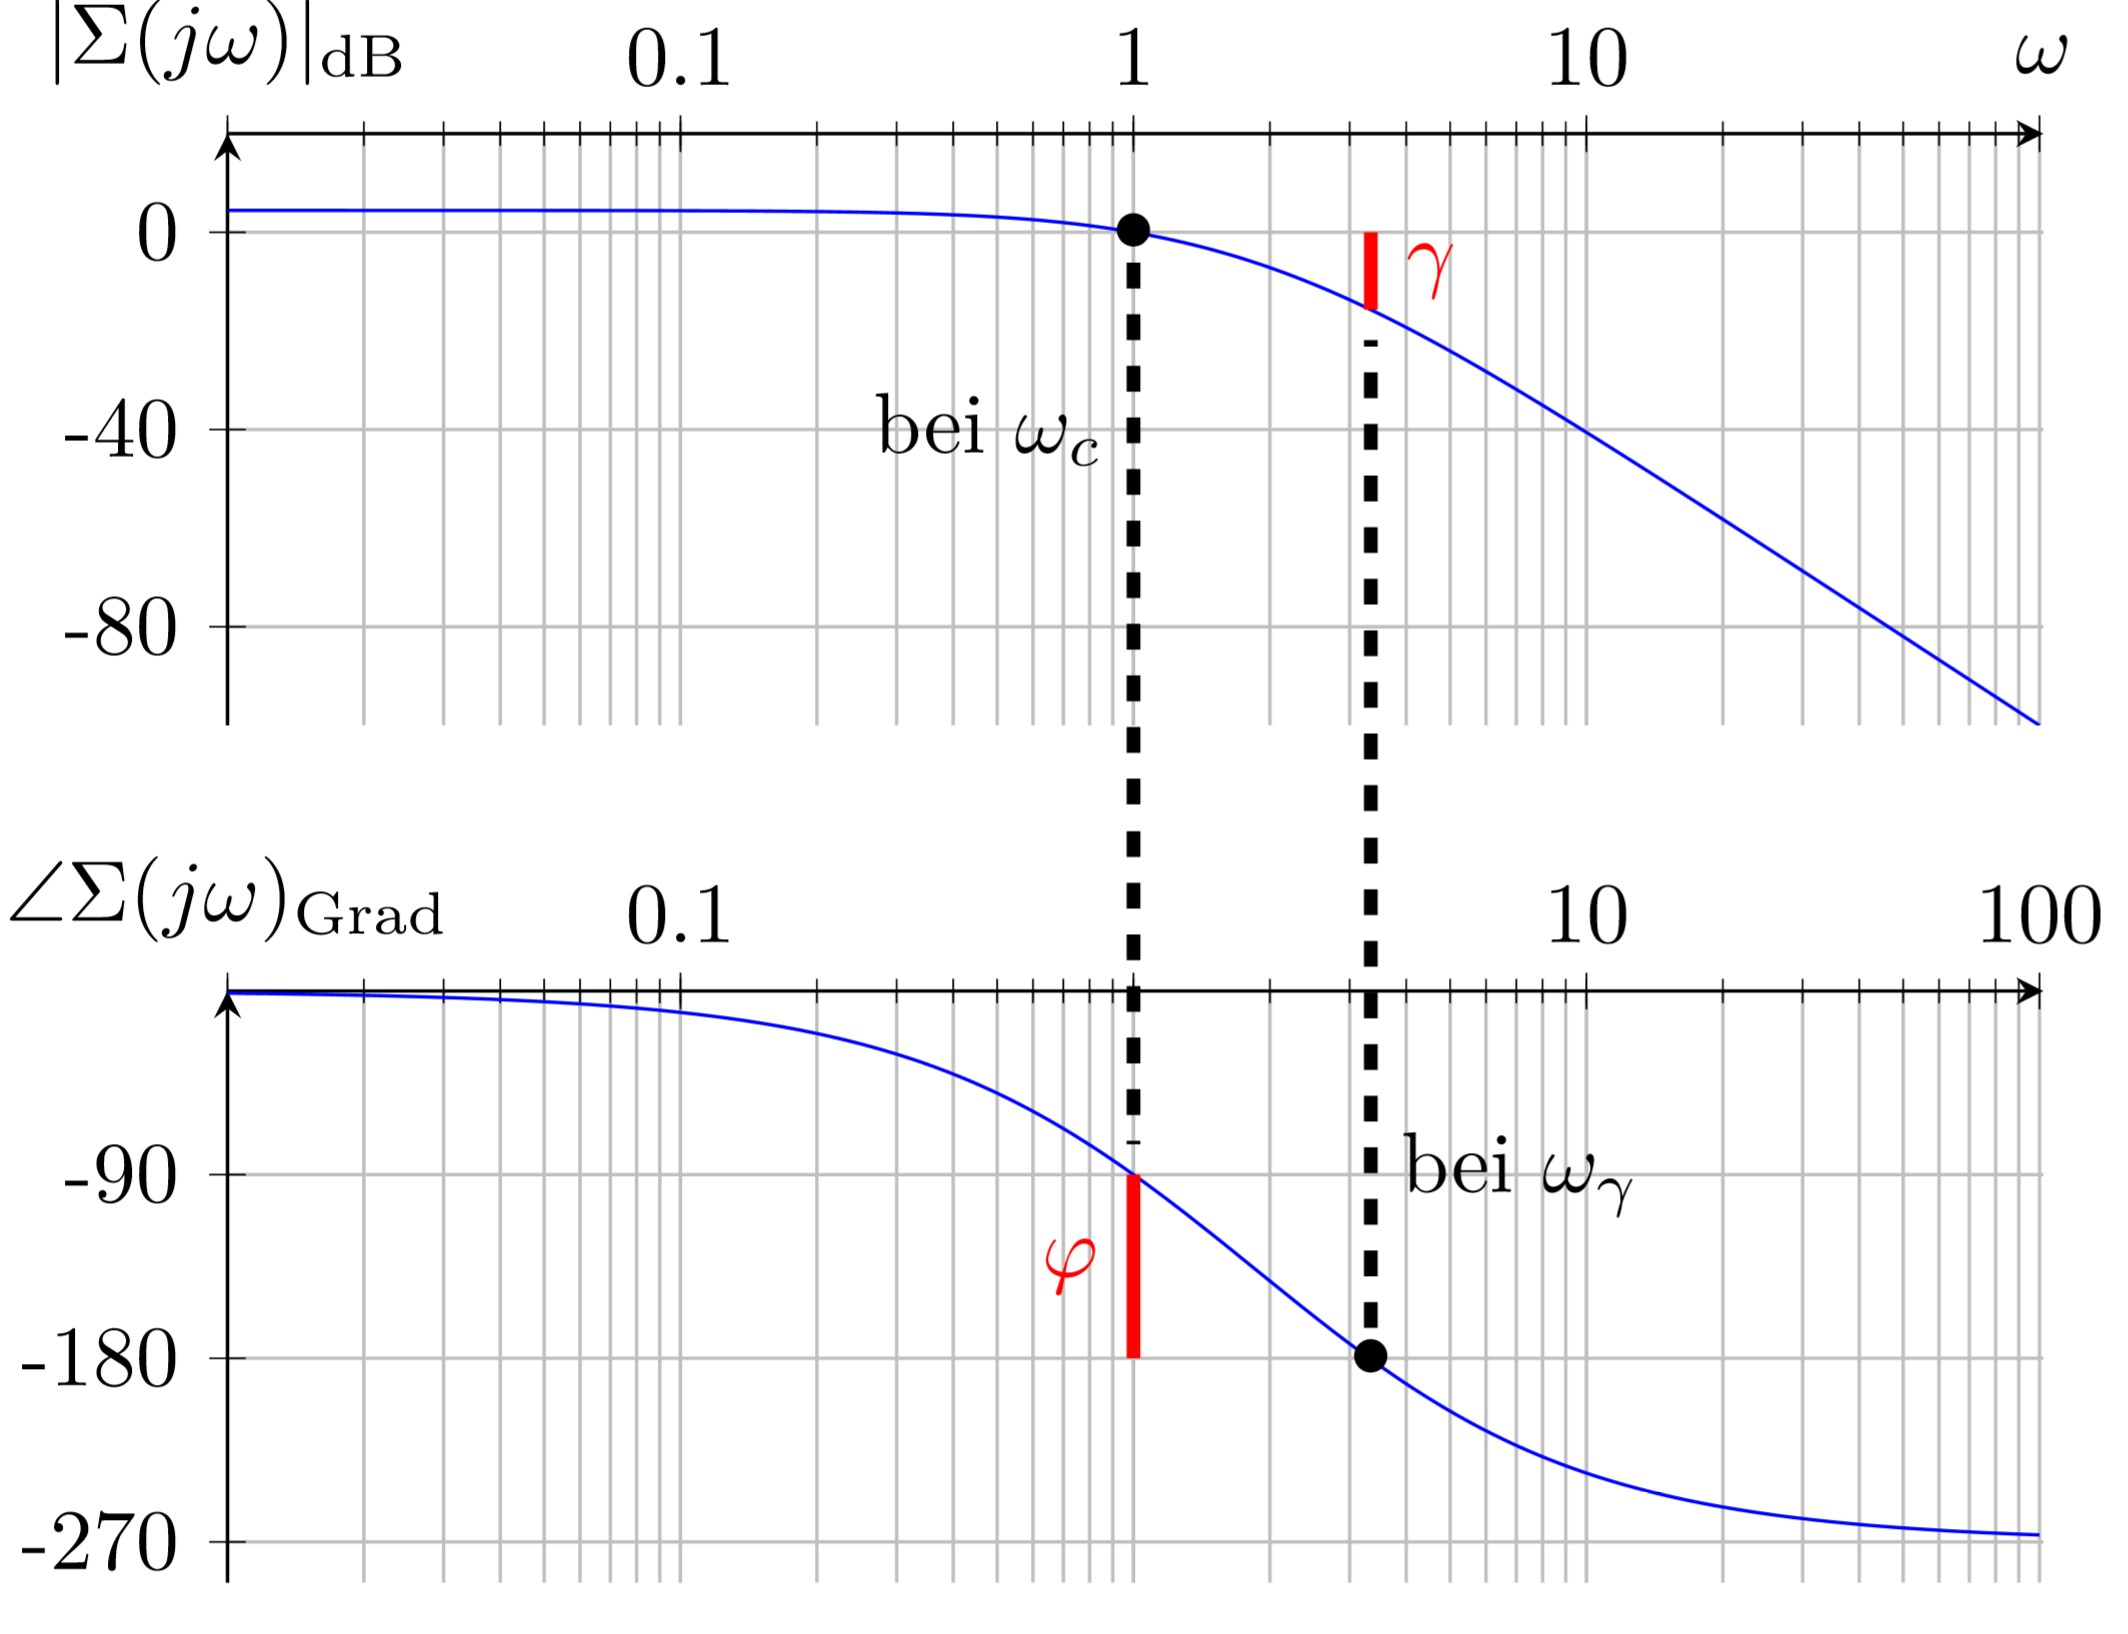
\includegraphics[width=0.7\linewidth]{images/07/reserven_im_bode.jpg}
            \end{center}
    \subsection{Robustes Nyquist Theorem}
        Ein wahres Modell der linearen und zeitinvarianten Regelstrecke $P_t(s)$ existiert, ist aber wegen Modellierungsunsicherheit nicht bekannt. Stattdessen wurde ein Nominalmodell der Regelstrecke $P(s)$ und eine zugehörige multiplikative Unsicherheitübertragungsfunktion $W_2(s)$ gefunden. Der Regler $ C(s)$ ist exakt bekannt. die wahre Kreisverstärkung des Systems $L_t(s) = P_t(s) \cdot C(s)$ ist Teil der Menge $\mathcal{S}_\mathcal{L}$:
        \[\mathcal{S}_\mathcal{L} = \{P(s)\cdot C(s) \cdot (1+\Delta \cdot W_2(s))\}\]
        \[\textrm{mit} |\Delta| \leq 1, \angle\Delta \in [-\pi,\pi]\]
        
        Es wird angenommen, dass $L(s)$ und $L_t(s)$ dieselbe Anzahl instabile $(n+)$ und stabile $(n_0)$ Pole haben.
        
        \subsubsection{Robustes Stabilitätskriterium von Nyquist}
            Das robuste Stabilitätskriterium von Nyquist wird aus dem nominalen Nyquist-Stabilitätskriterium abgeleitet: Falls nämlich das nominale Nyquist-Stabilitätskriterium für jedes $ L_t(j\omega)\in\mathcal{S}_\mathcal{L} $ in Gl.(3) erfüllt ist, dann ist der Regelkreis garantiert asymptotisch stabil.
          
            Umsetzung des robusten Stabilitätskriteriums: Durch betrachten der grössen Modellunsicherheit, d.h. mit $|\Delta|=1$ und für alle möglichen Richtungen (Phasen) von $\Delta$ beschränken wir unsere Überlegung auf den schlimmst möglichen Fall, d.h. 
            \[L_t(s) = L(s) + L(s)\cdot W_2(s)\]
            $\Rightarrow$ Kreise die durch $(0,0)$ gehen.
 \vfill\null\columnbreak          
            Um zusätzliche Umkreisungen des Punktes (-1+0j) garantiert zu verhindern, darf der Unsicherheitsradius \textcolor{red}{$|L(j\omega)\cdot W_2(j\omega)|$} nie grösser als \textcolor{blue}{$|1+L(j\omega)|$} werden. Daraus folgt das robuste Stabilitätskriterium nach Nyquist:
            
            \[|L(j\omega)\cdot W_2(j\omega)| < |1+L(j\omega)|,\forall\omega\in[0,\infty)\]
            
            \begin{center}
                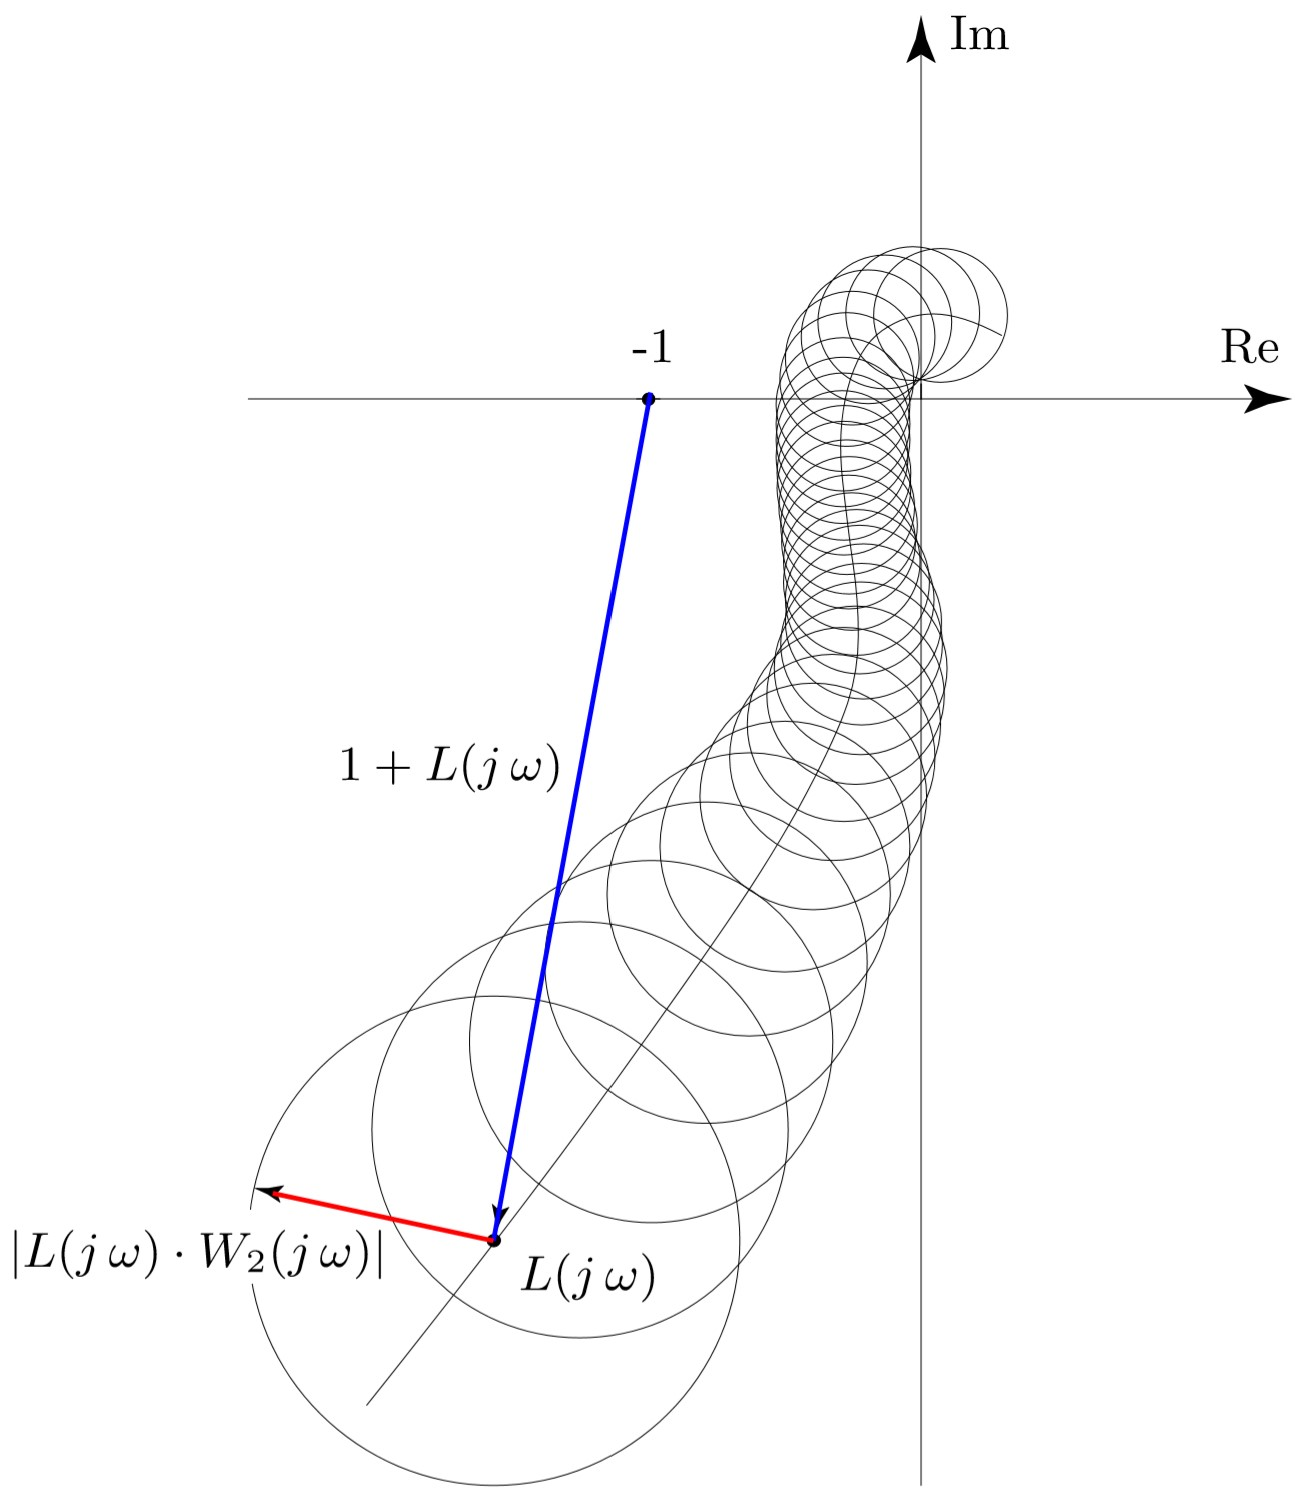
\includegraphics[width = 0.6\linewidth]{images/07/Robustes_nyq_Stabkrit.jpg}
            \end{center}